\begin{figure}
	\centering
	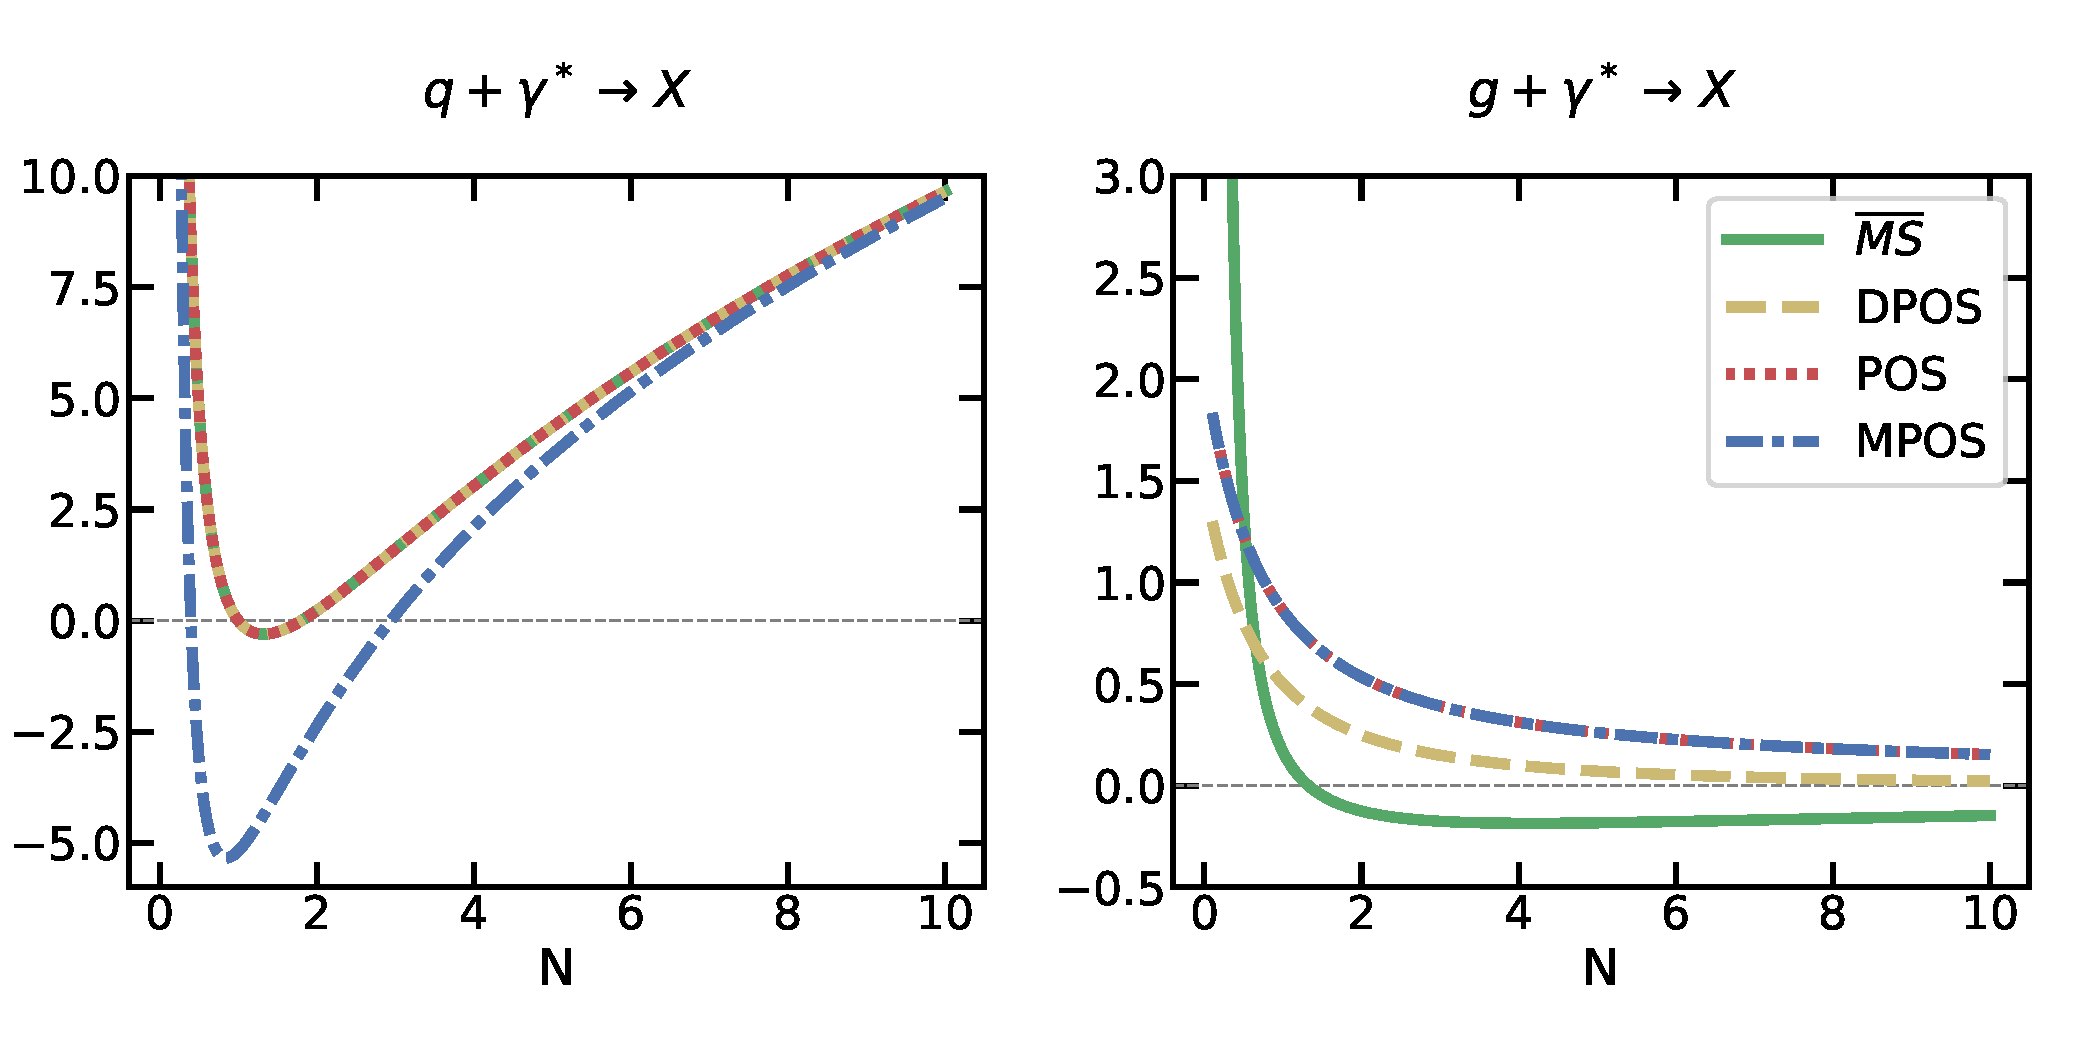
\includegraphics[width=0.7\textwidth]{ch-qcd/dis}
	\caption{The \acrfull{dis} process.}
	\label{fig:qcd/dis}
\end{figure}

The Deep Inelastic Scattering process is the scattering of a lepton over an
hadron component, mediated by an \ew boson \cref{fig:qcd/dis}.
%
The leptonic part does not couple directly to \qcd , thus the $\alpha_s$
corrections do apply only to the hadronic side (at \lo \ew), and the \ew boson
can be seen as emitted from the incoming lepton and absorbed into the hadron.
%
In this picture the process can be interpreted as the scattering of an
off-shell \ew boson over an hadron, probing the hadron composition.

\subsection{Kinematics}

The following kinematic variables are often used in the following:

\begin{align}
	Q^2   & = - q^2                       \\
	M_h^2 & = p^2                         \\
	\nu   & = q \cdot p                   \\
	x     & = \frac{Q^2}{2\nu}            \\
	y     & = \frac{q \cdot p}{k \cdot p}
\end{align}

so $M_h$is the mass of the scattered hadron, while $x$and
$y$are Bjorken variables.

\subparagraph{Hadronic vs Partonic} Notice that the variables listed here
are all **hadronic**, so $x$is not the partonic momentum fraction (it is only
at \lo , because the coefficient function is a $\delta$).
In order to avoid confusion the coefficient function variable will be called
$z$, and thus the partonic momentum fraction will be $x/z$.
